\chapter{Clean Architecture}

%% Plugins (DB / GUI) -> Adapters (Presenters, Controllers, Gateways) -> Application Code (Use Cases) -> Domain Code (Entities) -> Abstraction Code (Generic Entities (mathematische Konzepte))
%% Abstraction Code: 
%%  Mathematische Konzepte (z.B. Matrizen)
%%  Algorithmen und Datenstrukturen (z.B. Zelluläre Automaten)
%%  Abstrahierte Muster (z.B. Quantitäten)
%%  !!!!!Häufig nicht notwendig!!!!
%% 
%% Domain Code:
%%  Entities 
%%  Implementiert organisationsweit gültige Geschäftslogik
%%  Sollte sich am seltensten ändern
%% 
%% Application Code:
%%  Use Cases
%%  Implementiert die anwendungsspezifische Geschäftslogik
%%  Steuert den Fluss der Daten und Aktionen von und zu den Entities
%% 
%% Adapters:
%%  Diese Schicht vermittelt Aufrufe und Daten an die inneren Schichten
%%  Formatkonvertierungen
%%  Oftmals nur einfache Datenstrukturen, die hin- und hergereicht werden
%%  Anti-Corruption Layer
%% 
%% Plugins:
%%  Diese Schicht greift grundsätzlich nur auf die Adapter zu
%%  Enthält Frameworks, Datentransportmittel und andere Werkzeuge (Datenbank, API)
%%  Wir versuchen, hier möglichst wenig Code zu schreiben
%%  Hauptsächlich Delegationscode, der an die Adapter weiterleitet
%% 
%% Grundregeln der Clean Architecture
%%  ● Der Anwendungs- und Domaincode ist frei von Abhängigkeiten
%%  ● Sämtlicher Code kann eigenständig verändert werden
%%  ● Sämtlicher Code kann unabhängig von Infrastruktur kompiliert und ausgeführt werden
%%  ● Innere Schichten definieren Interfaces, äußere Schichten implementieren diese
%%  ● Die äußeren Schichten koppeln sich an die inneren Schichten (Richtung Zentrum)

%% Konkrete Umsetzung
%% ●Nicht alle Klassenin einem Projekt
%% ●Schichtenbildung überPackages ist in Ordnung
%% ●Aber: keine Überprüfungdurch den Compiler
%% ●Lieber mehrere Projekte(„Multi-Projekt“)
%% ●Compiler findet nur Klassen–im eigenen Projekt–in referenzierten Projekten
%% Maven parent Pom

%% Ziel der Clean Architecture
%% Das Ziel der Clean Architecture ist, Code nur von langlebigerem Code abhängig zu machen
%% Wenn sich Technologien ändern müssen, kann die Anwendung unverändert bleiben

\section{Schichtarchitektur planen und begründen}

\begin{figure}[htbp]
    \centering
    \fbox{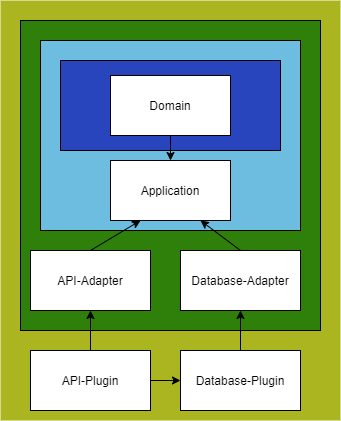
\includegraphics[width=6cm]{schichtarchitektur}} %% TODO Pfeile fixen
    \caption{\label{flutter-1} Schichtarchitektur}
\end{figure}
%% genauer erklären warum es aufgespalten wurde!!!!
Die Schichtarchitektur wurde nach den Regeln der Clean Architecture in vier Schichten unterteilt:
\begin{itemize}
    \item Plugin
    \item Adapter
    \item Application
    \item Domain
\end{itemize}
\newpage
Zudem wurden in diesen Schichten die fundamentalen Grundregeln beachtet:
\begin{itemize}
    \item Der Anwendungs- und Domaincode ist frei von Abhängigkeiten
    \item Sämtlicher Code kann eigenständig verändert werden
    \item Sämtlicher Code kann unabhängig von Infrastruktur kompiliert und ausgeführt werden
    \item Innere Schichten definieren Interfaces, äußere Schichten implementieren diese
    \item Die äußeren Schichten koppeln sich an die inneren Schichten in Richtung Zentrum
\end{itemize}
Die wichtigste dieser Regeln ist dabei die Richtung von außen nach innen, wodurch die äußeren Schichten immer nur von inneren Schichten abhängig sind.
Somit können äußere Schichten jederzeit ausgetauscht oder angepasst werden ohne dabei innere Schichten zu beeinflussen.


Die Plugin-Schicht wurde nochmals in API und Datenbank aufgeteilt um die übersichtlichkeit des Codes etwas zu erhöhen.
Zudem wird dadurch ermöglicht nicht nur verschiedene Datenstrukturen zwischen Plugin- und Domaincode sondern auch zwischen API und Datenbank zu haben.
Ein wichtiges Beispiel hierfür ist der User, welcher in der Datenbank ein Passwort besitzt aber in der API ohne dieses ausgegeben werden soll.
Die Plugin Schicht ist die äußerste Schicht und hat somit als einzige externe Abhängigkeiten, neben den Test-Dependencies welche von allen benötigt werden.
Was ja auch eine der fundamentalen Regeln der Clean Architecture ist.
Sie enthält allgemein also Frameworks, Datentransportmittel und andere Werkzeuge.
In diesem Fall befinden sich hier die Datenbank Implementierung und das API Framework.
Die Schicht ist aber vom Funktionsumfang nur für die Delegation der externen Anfragen an die Adapter zuständig.



Die Adapter-Schicht wurde auch in API und Datenbank aufgeteilt und konvertiert die jeweiligen Objekt Datenstrukturen aus API und Datenbank in die Strukturen der inneren Schichten.
Die Adapter rufen dann Funktionen aus der Application-Schicht mit den konvertierten Daten auf und dient als ein Anti-Corruption Layer zwischen den Technischen Schichten und der Geschäftslogik.



In der Application-Schicht liegt dann die eigentliche anwendungsspezifische Geschäftslogik und hier werden API und Datenbank zusammen geführt.
Hier werden unter anderem Domain Service Interfaces Implementiert und die Funktionen der Repositories und Aggregates aufgerufen.
Die steuert also sozusagen den Fluss der Daten und Aktionen von und zu den Aggregaten und somit auch den darin enthaltenen Entities.




In der Domain Schicht befinden sich die Entities, Value Objects, Aggregate, Repositories und Domain Services auf welche die Application Schicht zugreift.
Hier liegt also die organisationsweit gültige und somit anwendungsunabhänige Geschäftslogik, dies dient dem Ziel diese in Zukunft zum Beispiel in anderen Anwendungen verwenden zu können.
Die Repository-Interfaces welche von darunter liegenden Schichten implementiert werden erlauben der Application und Domain Schicht auf die Persistierung zuzugreifen ohne dabei von deren Implementierung
abhängig zu sein indem eine Inversion of Control erzeugen wird.




Die Abstraction Schicht, welche die innerste Schicht ist, wurde nicht Implementiert, da es sich hierbei um eine Schicht handelt welche zum Beispiel allgemeine Mathematische Konzepte,
Algorithmen oder Abstrahierte Muster beeinhaltet. Diese kommen in dieser Domäne aber nicht vor wodurch diese Schicht in diesem Fall keinen Sinn hätte.